% =====================================================================
%  IN6049 --- Forecasting and Regression Analysis
%  Week 4: Multiple Regression I and the Hat Matrix --- Tips dataset
%
%  Built from template/slides-template.tex (Boadilla + seahorse, 16:9).
%  Title slide + 4 content slides.  Numbers come from Assigment_4.ipynb;
%  figures are its exported PNGs (images/ -> fig_*.png here).
%
%  Compiles on Overleaf with the default pdfLaTeX engine.
%  Upload alongside: fig_plane.png , fig_resid.png , fig_lev.png , fig_infl.png
% =====================================================================
\documentclass[aspectratio=169,11pt]{beamer}

\usetheme{Boadilla}
\usecolortheme{seahorse}
\setbeamertemplate{navigation symbols}{}

\usepackage[utf8]{inputenc}
\usepackage[T1]{fontenc}
\usepackage{booktabs}
\usepackage{amsmath}
\usepackage{graphicx}
\usepackage{url}

% Emphasis lead-in: bold + structure colour.  Use as \key{Finding.} text...
\newcommand{\key}[1]{\textbf{\structure{#1}}}

% Figure placeholder, so the template compiles with no image files.
% Replace each use by  \includegraphics[width=0.9\linewidth]{@@ file @@}
% (vector PDF preferred; PNG is fine).
\newcommand{\figbox}[2]{%
  \fbox{\parbox[c][#2][c]{#1}{\centering\scriptsize\color{gray}@@ figure @@}}}

% ---------------------------------------------------------------------
\title[Multiple regression and the hat matrix]{Multiple Regression and the Hat Matrix --- Restaurant Tips}
\subtitle{From one predictor to two, and the matrix behind the fit}
\author[Jie Dong, Elivier Reyes]{Jie Dong, Elivier Reyes}
\date[IN6049]{}

\begin{document}

% ===================== TITLE ========================================
\begin{frame}
  \titlepage
  \vspace{-1.2em}
  \begin{center}
    \small\urlstyle{same}\url{https://github.com/HelloJJJie/Assignment-Forecast-and-Analysis-of-Regression.git}

    \vspace{1.2em}
    A dataset of $n=244$ restaurant bills --- what do the bill \emph{and} the party
    size tell us about the tip?
  \end{center}
\end{frame}

% ===================== 1. MODEL AND FIT =============================
\begin{frame}{1. The model in matrix form, and the fit}
  \begin{columns}[T]
  \begin{column}{0.54\textwidth}
    \small
    \key{Data.} $Y=$ tip, $X_1=$ bill (USD), $X_2=$ party size
    ($1$--$6$); $p=3$.

    \vspace{0.1em}
    \[
      \mathbf Y=\mathbf X\boldsymbol\beta+\boldsymbol\varepsilon
      \;\Rightarrow\;
      \mathbf b=(\mathbf X'\mathbf X)^{-1}\mathbf X'\mathbf Y
    \]
    \vspace{-1.3em}

    $\hat Y=0.669+0.0927X_1+0.1926X_2$, $MSE=1.027$ ($241$ df).

    \vspace{0.2em}
    {\scriptsize
    \begin{tabular}{@{}lrrrr@{}}
      \toprule
       & $b$ & $s\{b\}$ & $t^{*}$ & $P$ \\
      \midrule
      intercept & $0.6689$ & $0.1936$ & $3.46$  & $6.5\times10^{-4}$ \\
      total bill & $0.0927$ & $0.0091$ & $10.17$ & $1.9\times10^{-20}$ \\
      size      & $0.1926$ & $0.0853$ & $2.26$  & $0.025$ \\
      \bottomrule
    \end{tabular}}


    \vspace{0.2em}
    \small
    \begin{itemize}
      \item \key{Partial effect:} $b_1$ is $11.7\%$ below the simple slope
            $0.1050$ ($r_{X_1X_2}=0.598$).
      \item \key{Overall $F$:} $105.95>F(0.95;2,241)=3.03$, reject
            $\beta_1=\beta_2=0$; $R^2=0.468$, $R^2_a=0.463$ (bill alone: $0.457$).
    \end{itemize}
  \end{column}
  \begin{column}{0.46\textwidth}
    \centering
    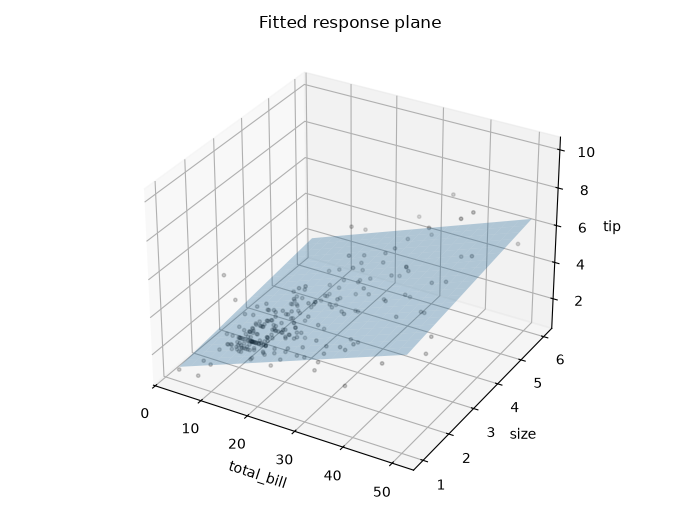
\includegraphics[width=0.95\linewidth]{fig_plane.png}

    \vspace{-0.2em}
    {\scriptsize The response surface is a plane; each coefficient holds the
     other predictor fixed.}
  \end{column}
  \end{columns}
\end{frame}

% ===================== 2. PREDICTION AND DIAGNOSTICS ================
\begin{frame}{2. Prediction and diagnostics}
  \begin{columns}[T]
  \begin{column}{0.46\textwidth}
    \small
    \key{Estimation at} $\mathbf X_h=(1,20,3)$ (\$20 bill, party of 3);
    $s^2\{\hat Y_h\}=MSE\,\mathbf X_h'(\mathbf X'\mathbf X)^{-1}\mathbf X_h$:

    \vspace{0.2em}
    {\scriptsize
    \begin{tabular}{@{}lr@{}}
      \toprule
      fitted tip $\hat Y_h$   & $3.10$ \\
      $95\%$ CI, mean tip     & $[2.955,\,3.247]$ \\
      $95\%$ PI, one new tip  & $[1.099,\,5.103]$ \\
      \bottomrule
    \end{tabular}}

    \vspace{0.4em}
    \small
    \begin{itemize}
      \item \key{Constant variance rejected:} Breusch--Pagan $\chi^2=92.2$,
            $P=9.4\times10^{-21}$; residual sd $0.68/0.76/1.42$ by thirds of
            fitted value.
      \item \key{Normality rejected:} plot $r=0.982$ vs.\ critical $0.994$.
      \item \key{No interaction signal:} $\mathrm{corr}(e,X_1X_2)=+0.007$.
    \end{itemize}
  \end{column}
  \begin{column}{0.54\textwidth}
    \centering
    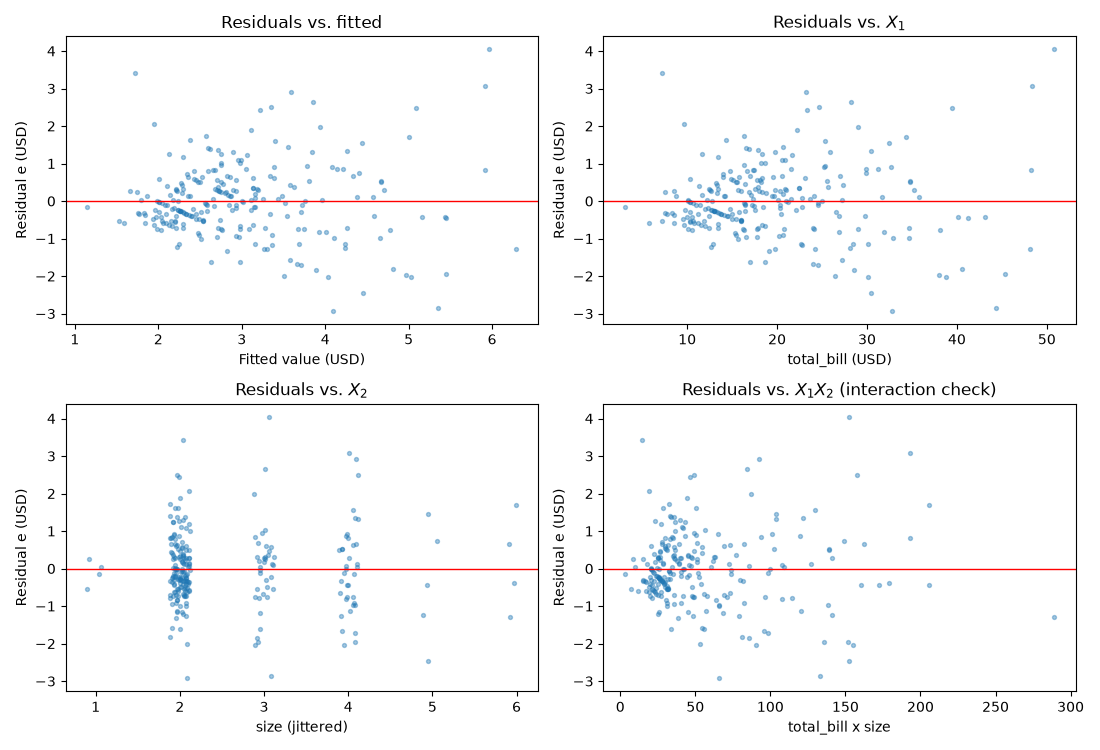
\includegraphics[width=0.98\linewidth]{fig_resid.png}

    \vspace{-0.2em}
    {\scriptsize The funnel is the same one seen with a single predictor:
     the prediction interval has constant width, the scatter does not.}
  \end{column}
  \end{columns}
\end{frame}

% ===================== 3. HAT MATRIX AND LEVERAGE ===================
\begin{frame}{3. The hat matrix and leverage}
  \begin{columns}[T]
  \begin{column}{0.52\textwidth}
    \small
    \[
      \hat{\mathbf Y}=\underbrace{\mathbf X(\mathbf X'\mathbf X)^{-1}\mathbf X'}_{\mathbf H}\,\mathbf Y,
      \qquad \mathbf e=(\mathbf I-\mathbf H)\mathbf Y
    \]
    $\mathbf H$ is $244\times244$: a \emph{projection} of $\mathbf Y$ onto the
    columns of $\mathbf X$. Checked numerically (max deviation $<10^{-13}$):
    \begin{itemize}
      \item \key{Symmetric and idempotent:} $\mathbf H'=\mathbf H$,\; $\mathbf H^2=\mathbf H$;
            $\mathbf H\mathbf X=\mathbf X$, $\mathbf X'\mathbf e=\mathbf 0$.
      \item $\operatorname{tr}\mathbf H=3=p$, so the average leverage is
            $p/n=0.0123$; $SSTO=SSR+SSE$ ($465.2=217.7+247.6$).
      \item \key{Leverage} $h_{ii}$: $22$ of $244$ cases exceed $2p/n=0.0246$.
            The largest: bill $\$50.81$ ($h=0.071$); parties of $6$ also rank high.
      \item $s^2\{\hat Y_i\}=MSE\cdot h_{ii}$: the mean-response interval
            is widest where leverage is highest.
    \end{itemize}
  \end{column}
  \begin{column}{0.48\textwidth}
    \centering
    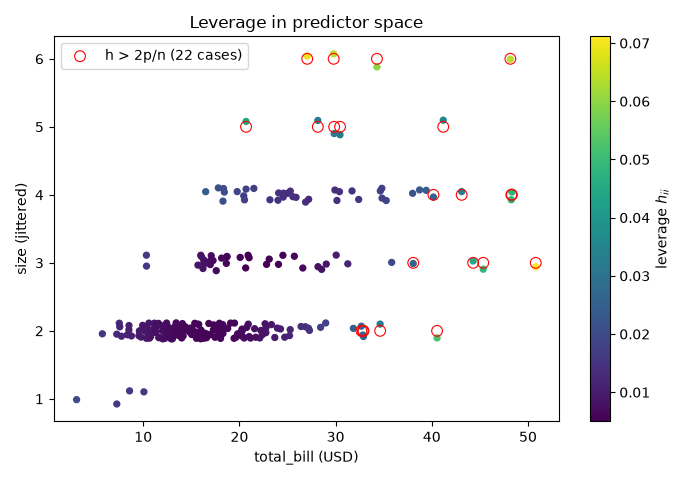
\includegraphics[width=0.92\linewidth]{fig_lev.png}

    \vspace{-0.2em}
    {\scriptsize Leverage is distance in predictor space, not in $Y$. A point can
     lie inside each variable's range and still outside the cloud: $(50,\,1)$ has
     $h=0.138$, about $2\times$ the largest observed.}
  \end{column}
  \end{columns}
\end{frame}

% ===================== 4. INFLUENCE =================================
\begin{frame}{4. Residual variance and influence}
  \begin{columns}[T]
  \begin{column}{0.46\textwidth}
    \centering
    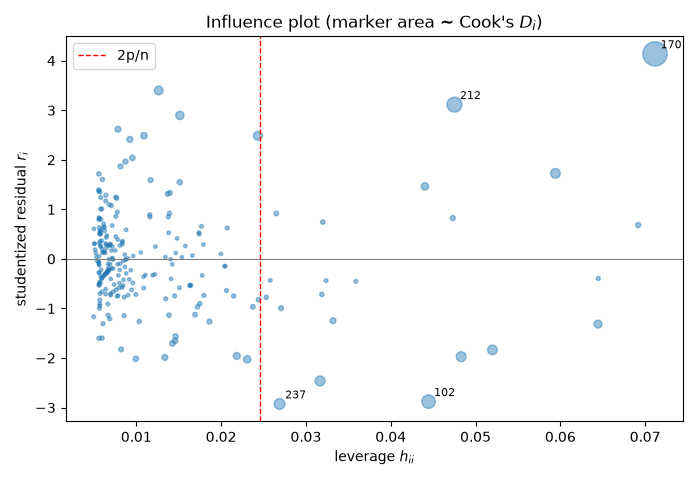
\includegraphics[width=0.88\linewidth]{fig_infl.png}

    \vspace{0.2em}
    {\scriptsize\setlength{\tabcolsep}{3pt}
    \begin{tabular}{@{}lrrr@{}}
      \toprule
      Drop rows $170,212,102$ & $b_0$ & $b_1$ & $b_2$ \\
      \midrule
      change & $+15.6\%$ & $-12.0\%$ & $+19.2\%$ \\
      \bottomrule
    \end{tabular}}
  \end{column}
  \begin{column}{0.54\textwidth}
    \small
    \begin{itemize}
      \item $\operatorname{Var}\{e_i\}=\sigma^2(1-h_{ii})$: high-leverage points
            have \emph{smaller} residual variance. The studentized residual
            $r_i=e_i/\sqrt{MSE(1-h_{ii})}$ treats cases fairly --- here it barely
            moves ($r_i/e^{*}_i\in[1.003,\,1.038]$) because all $h_{ii}$ are small.
      \item \key{Leverage is only potential influence.} Row $170$ (bill
            $\$50.81$, tip $\$10$) combines the highest leverage with the
            largest residual: $r=4.14$, Cook's $D=0.437$ (next: $0.161$).
      \item Dropping the three cases with the largest $D$ shifts the
            coefficients by $12$--$19\%$.
    \end{itemize}

    \vspace{0.1em}
    \key{Takeaway.} The two-predictor model passes the overall $F$ test but
    explains only $47\%$ of the variance, fails constant variance and
    normality, and three cases move the coefficients by $12$--$19\%$.
  \end{column}
  \end{columns}
\end{frame}

\end{document}
